\documentclass[tikz,border=3pt]{standalone}
\usepackage[utf8]{inputenc}
\usepackage[T1]{fontenc}
\usepackage{lmodern}
\renewcommand{\familydefault}{\sfdefault}
\usepackage{sansmath}\sansmath
\usepackage{chemfig}
\usepackage{pgfplots}\pgfplotsset{compat=1.18,/pgf/number format/use comma,/pgf/number format/1000 sep={.}}
\usetikzlibrary{arrows.meta,calc,positioning,decorations.pathmorphing,patterns}
% paleta del sitio
\definecolor{nar}{HTML}{E8680C}\definecolor{narc}{HTML}{FFB35C}\definecolor{hielo}{HTML}{FFF3E8}
\definecolor{tinta}{HTML}{1D1D1F}\definecolor{gris}{HTML}{6E6E73}\definecolor{lila}{HTML}{7C5CF0}
\definecolor{azul}{HTML}{2F6FD6}\definecolor{menta}{HTML}{17A673}\definecolor{coral}{HTML}{E8342A}
\tikzset{cel/.style={draw=gris,fill=hielo,line width=0.9pt},nuc/.style={draw=gris!70,line width=0.6pt},
fib/.style={gris!55,line width=0.35pt},eti/.style={font=\footnotesize,text=tinta,align=center},
num/.style={circle,draw=nar,fill=white,text=nar,font=\small\bfseries,inner sep=1.2pt,minimum size=13pt},
fl/.style={-{Stealth[length=2.6mm]},gris,line width=0.9pt}}
\begin{document}
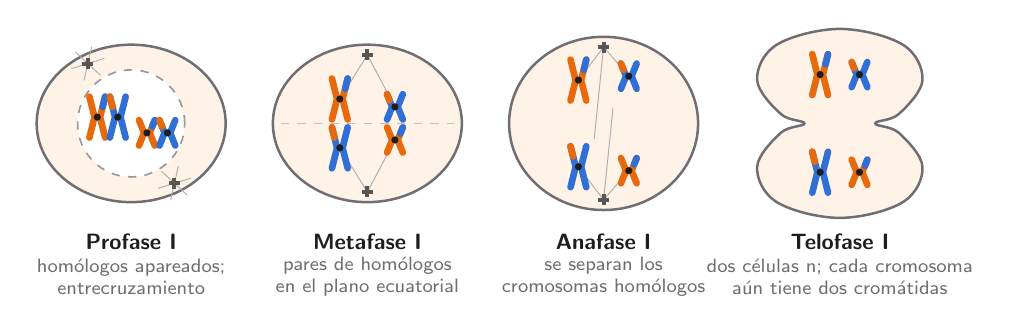
\begin{tikzpicture}[font=\small]
\draw[cel] (0,0) ellipse (1.2 and 1);
\draw[nuc,fill=white,dashed] (0,0) circle (0.68);
\begin{scope}[shift={(-0.43,0.08)},rotate=0]\draw[nar,line width=2.4pt,line cap=round,line join=round] (-0.1,0.26)--(-0.035,0)--(-0.1,-0.26);\end{scope}
\begin{scope}[shift={(-0.43,0.08)},rotate=0]\draw[nar,line width=2.4pt,line cap=round,line join=round] (0.1,0.26)--(0.035,0)--(0.1,-0.26);\draw[azul,line width=2.4pt,line cap=round] (0.1,0.26)--(0.068,0.13);\end{scope}
\fill[tinta] (-0.43,0.08) circle (1.3pt);
\begin{scope}[shift={(-0.17,0.08)},rotate=0]\draw[azul,line width=2.4pt,line cap=round,line join=round] (-0.1,0.26)--(-0.035,0)--(-0.1,-0.26);\draw[nar,line width=2.4pt,line cap=round] (-0.1,0.26)--(-0.068,0.13);\end{scope}
\begin{scope}[shift={(-0.17,0.08)},rotate=0]\draw[azul,line width=2.4pt,line cap=round,line join=round] (0.1,0.26)--(0.035,0)--(0.1,-0.26);\end{scope}
\fill[tinta] (-0.17,0.08) circle (1.3pt);
\begin{scope}[shift={(0.2,-0.12)},rotate=0]\draw[nar,line width=2.4pt,line cap=round,line join=round] (-0.1,0.16)--(-0.035,0)--(-0.1,-0.16);\end{scope}
\begin{scope}[shift={(0.2,-0.12)},rotate=0]\draw[nar,line width=2.4pt,line cap=round,line join=round] (0.1,0.16)--(0.035,0)--(0.1,-0.16);\draw[azul,line width=2.4pt,line cap=round] (0.1,0.16)--(0.068,0.08);\end{scope}
\fill[tinta] (0.2,-0.12) circle (1.3pt);
\begin{scope}[shift={(0.46,-0.12)},rotate=0]\draw[azul,line width=2.4pt,line cap=round,line join=round] (-0.1,0.16)--(-0.035,0)--(-0.1,-0.16);\draw[nar,line width=2.4pt,line cap=round] (-0.1,0.16)--(-0.068,0.08);\end{scope}
\begin{scope}[shift={(0.46,-0.12)},rotate=0]\draw[azul,line width=2.4pt,line cap=round,line join=round] (0.1,0.16)--(0.035,0)--(0.1,-0.16);\end{scope}
\fill[tinta] (0.46,-0.12) circle (1.3pt);
\draw[fib] (-0.55,0.76)--(-0.34,0.825);
\draw[fib] (-0.55,0.76)--(-0.501,0.975);
\draw[fib] (-0.55,0.76)--(-0.711,0.91);
\draw[fib] (-0.55,0.76)--(-0.76,0.695);
\draw[fib] (-0.55,0.76)--(-0.599,0.545);
\draw[fib] (-0.55,0.76)--(-0.389,0.61);
\draw[fib] (0.55,-0.76)--(0.76,-0.695);
\draw[fib] (0.55,-0.76)--(0.599,-0.545);
\draw[fib] (0.55,-0.76)--(0.389,-0.61);
\draw[fib] (0.55,-0.76)--(0.34,-0.825);
\draw[fib] (0.55,-0.76)--(0.501,-0.975);
\draw[fib] (0.55,-0.76)--(0.711,-0.91);
\fill[tinta!75] (-0.62,0.735) rectangle (-0.48,0.785);\fill[tinta!75] (-0.575,0.69) rectangle (-0.525,0.83);
\fill[tinta!75] (0.48,-0.785) rectangle (0.62,-0.735);\fill[tinta!75] (0.525,-0.83) rectangle (0.575,-0.69);
\draw[cel] (3,0) ellipse (1.2 and 1);
\draw[gris!45,dashed] (1.9,0)--(4.1,0);
\draw[fib] (3,0.87)--(2.65,0.31);
\draw[fib] (3,0.87)--(3.35,0.21);
\draw[fib] (3,-0.87)--(2.65,-0.31);
\draw[fib] (3,-0.87)--(3.35,-0.21);
\begin{scope}[shift={(2.65,0.31)},rotate=0]\draw[nar,line width=2.4pt,line cap=round,line join=round] (-0.1,0.26)--(-0.035,0)--(-0.1,-0.26);\end{scope}
\begin{scope}[shift={(2.65,0.31)},rotate=0]\draw[nar,line width=2.4pt,line cap=round,line join=round] (0.1,0.26)--(0.035,0)--(0.1,-0.26);\draw[azul,line width=2.4pt,line cap=round] (0.1,0.26)--(0.068,0.13);\end{scope}
\fill[tinta] (2.65,0.31) circle (1.3pt);
\begin{scope}[shift={(3.35,0.21)},rotate=0]\draw[azul,line width=2.4pt,line cap=round,line join=round] (-0.1,0.16)--(-0.035,0)--(-0.1,-0.16);\draw[nar,line width=2.4pt,line cap=round] (-0.1,0.16)--(-0.068,0.08);\end{scope}
\begin{scope}[shift={(3.35,0.21)},rotate=0]\draw[azul,line width=2.4pt,line cap=round,line join=round] (0.1,0.16)--(0.035,0)--(0.1,-0.16);\end{scope}
\fill[tinta] (3.35,0.21) circle (1.3pt);
\begin{scope}[shift={(2.65,-0.31)},rotate=0]\draw[azul,line width=2.4pt,line cap=round,line join=round] (-0.1,0.26)--(-0.035,0)--(-0.1,-0.26);\draw[nar,line width=2.4pt,line cap=round] (-0.1,0.26)--(-0.068,0.13);\end{scope}
\begin{scope}[shift={(2.65,-0.31)},rotate=0]\draw[azul,line width=2.4pt,line cap=round,line join=round] (0.1,0.26)--(0.035,0)--(0.1,-0.26);\end{scope}
\fill[tinta] (2.65,-0.31) circle (1.3pt);
\begin{scope}[shift={(3.35,-0.21)},rotate=0]\draw[nar,line width=2.4pt,line cap=round,line join=round] (-0.1,0.16)--(-0.035,0)--(-0.1,-0.16);\end{scope}
\begin{scope}[shift={(3.35,-0.21)},rotate=0]\draw[nar,line width=2.4pt,line cap=round,line join=round] (0.1,0.16)--(0.035,0)--(0.1,-0.16);\draw[azul,line width=2.4pt,line cap=round] (0.1,0.16)--(0.068,0.08);\end{scope}
\fill[tinta] (3.35,-0.21) circle (1.3pt);
\fill[tinta!75] (2.93,0.845) rectangle (3.07,0.895);\fill[tinta!75] (2.975,0.8) rectangle (3.025,0.94);
\fill[tinta!75] (2.93,-0.895) rectangle (3.07,-0.845);\fill[tinta!75] (2.975,-0.94) rectangle (3.025,-0.8);
\draw[cel] (6,0) ellipse (1.2 and 1.1);
\draw[fib] (6,0.97)--(5.68,0.55);
\draw[fib] (6,0.97)--(6.32,0.6);
\draw[fib] (6,-0.97)--(5.68,-0.55);
\draw[fib] (6,-0.97)--(6.32,-0.6);
\draw[fib] (6,0.97)--(5.88,-0.2);
\draw[fib] (6,-0.97)--(6.12,0.2);
\begin{scope}[shift={(5.68,0.55)},rotate=0]\draw[nar,line width=2.4pt,line cap=round,line join=round] (-0.1,0.26)--(-0.035,0)--(-0.1,-0.26);\end{scope}
\begin{scope}[shift={(5.68,0.55)},rotate=0]\draw[nar,line width=2.4pt,line cap=round,line join=round] (0.1,0.26)--(0.035,0)--(0.1,-0.26);\draw[azul,line width=2.4pt,line cap=round] (0.1,0.26)--(0.068,0.13);\end{scope}
\fill[tinta] (5.68,0.55) circle (1.3pt);
\begin{scope}[shift={(6.32,0.6)},rotate=0]\draw[azul,line width=2.4pt,line cap=round,line join=round] (-0.1,0.16)--(-0.035,0)--(-0.1,-0.16);\draw[nar,line width=2.4pt,line cap=round] (-0.1,0.16)--(-0.068,0.08);\end{scope}
\begin{scope}[shift={(6.32,0.6)},rotate=0]\draw[azul,line width=2.4pt,line cap=round,line join=round] (0.1,0.16)--(0.035,0)--(0.1,-0.16);\end{scope}
\fill[tinta] (6.32,0.6) circle (1.3pt);
\begin{scope}[shift={(5.68,-0.55)},rotate=0]\draw[azul,line width=2.4pt,line cap=round,line join=round] (-0.1,0.26)--(-0.035,0)--(-0.1,-0.26);\draw[nar,line width=2.4pt,line cap=round] (-0.1,0.26)--(-0.068,0.13);\end{scope}
\begin{scope}[shift={(5.68,-0.55)},rotate=0]\draw[azul,line width=2.4pt,line cap=round,line join=round] (0.1,0.26)--(0.035,0)--(0.1,-0.26);\end{scope}
\fill[tinta] (5.68,-0.55) circle (1.3pt);
\begin{scope}[shift={(6.32,-0.6)},rotate=0]\draw[nar,line width=2.4pt,line cap=round,line join=round] (-0.1,0.16)--(-0.035,0)--(-0.1,-0.16);\end{scope}
\begin{scope}[shift={(6.32,-0.6)},rotate=0]\draw[nar,line width=2.4pt,line cap=round,line join=round] (0.1,0.16)--(0.035,0)--(0.1,-0.16);\draw[azul,line width=2.4pt,line cap=round] (0.1,0.16)--(0.068,0.08);\end{scope}
\fill[tinta] (6.32,-0.6) circle (1.3pt);
\fill[tinta!75] (5.93,0.945) rectangle (6.07,0.995);\fill[tinta!75] (5.975,0.9) rectangle (6.025,1.04);
\fill[tinta!75] (5.93,-0.995) rectangle (6.07,-0.945);\fill[tinta!75] (5.975,-1.04) rectangle (6.025,-0.9);
\draw[cel] plot[smooth cycle,tension=0.6] coordinates {(9,1.2) (9.8,1) (10.05,0.55) (9.75,0.12) (9.45,0) (9.75,-0.12) (10.05,-0.55) (9.8,-1) (9,-1.2) (8.2,-1) (7.95,-0.55) (8.25,-0.12) (8.55,0) (8.25,0.12) (7.95,0.55) (8.2,1)};
\begin{scope}[shift={(8.75,0.62)},rotate=0]\draw[nar,line width=2.4pt,line cap=round,line join=round] (-0.1,0.26)--(-0.035,0)--(-0.1,-0.26);\end{scope}
\begin{scope}[shift={(8.75,0.62)},rotate=0]\draw[nar,line width=2.4pt,line cap=round,line join=round] (0.1,0.26)--(0.035,0)--(0.1,-0.26);\draw[azul,line width=2.4pt,line cap=round] (0.1,0.26)--(0.068,0.13);\end{scope}
\fill[tinta] (8.75,0.62) circle (1.3pt);
\begin{scope}[shift={(9.25,0.62)},rotate=0]\draw[azul,line width=2.4pt,line cap=round,line join=round] (-0.1,0.16)--(-0.035,0)--(-0.1,-0.16);\draw[nar,line width=2.4pt,line cap=round] (-0.1,0.16)--(-0.068,0.08);\end{scope}
\begin{scope}[shift={(9.25,0.62)},rotate=0]\draw[azul,line width=2.4pt,line cap=round,line join=round] (0.1,0.16)--(0.035,0)--(0.1,-0.16);\end{scope}
\fill[tinta] (9.25,0.62) circle (1.3pt);
\begin{scope}[shift={(8.75,-0.62)},rotate=0]\draw[azul,line width=2.4pt,line cap=round,line join=round] (-0.1,0.26)--(-0.035,0)--(-0.1,-0.26);\draw[nar,line width=2.4pt,line cap=round] (-0.1,0.26)--(-0.068,0.13);\end{scope}
\begin{scope}[shift={(8.75,-0.62)},rotate=0]\draw[azul,line width=2.4pt,line cap=round,line join=round] (0.1,0.26)--(0.035,0)--(0.1,-0.26);\end{scope}
\fill[tinta] (8.75,-0.62) circle (1.3pt);
\begin{scope}[shift={(9.25,-0.62)},rotate=0]\draw[nar,line width=2.4pt,line cap=round,line join=round] (-0.1,0.16)--(-0.035,0)--(-0.1,-0.16);\end{scope}
\begin{scope}[shift={(9.25,-0.62)},rotate=0]\draw[nar,line width=2.4pt,line cap=round,line join=round] (0.1,0.16)--(0.035,0)--(0.1,-0.16);\draw[azul,line width=2.4pt,line cap=round] (0.1,0.16)--(0.068,0.08);\end{scope}
\fill[tinta] (9.25,-0.62) circle (1.3pt);
\node[eti] at (0,-1.5) {\textbf{Profase I}};
\node[eti,font=\scriptsize,text=gris] at (0,-1.95) {homólogos apareados;\\entrecruzamiento};
\node[eti] at (3,-1.5) {\textbf{Metafase I}};
\node[eti,font=\scriptsize,text=gris] at (3,-1.95) {pares de homólogos\\en el plano ecuatorial};
\node[eti] at (6,-1.5) {\textbf{Anafase I}};
\node[eti,font=\scriptsize,text=gris] at (6,-1.95) {se separan los\\cromosomas homólogos};
\node[eti] at (9,-1.5) {\textbf{Telofase I}};
\node[eti,font=\scriptsize,text=gris] at (9,-1.95) {dos células n; cada cromosoma\\aún tiene dos cromátidas};
\end{tikzpicture}
\end{document}
